\documentclass{article}

% if you need to pass options to natbib, use, e.g.:
%     \PassOptionsToPackage{numbers, compress}{natbib}
% before loading neurips_2019

% ready for submission
% \usepackage{neurips_2019}

% to compile a preprint version, e.g., for submission to arXiv, add add the
% [preprint] option:
    \usepackage[preprint]{neurips_2019}

% to compile a camera-ready version, add the [final] option, e.g.:
% \usepackage[final]{neurips_2019}

% to avoid loading the natbib package, add option nonatbib:
%     \usepackage[nonatbib]{neurips_2019}

\usepackage[utf8]{inputenc} % allow utf-8 input
\usepackage[T1]{fontenc}    % use 8-bit T1 fonts
\usepackage{hyperref}       % hyperlinks
\usepackage{url}            % simple URL typesetting
\usepackage{booktabs}       % professional-quality tables
\usepackage{caption}

% \DeclareCaptionLabelFormat{andtable}{#1~#2  \&  \tablename~\thetable}
\DeclareCaptionLabelFormat{andfigure}{#1~#2  \&  \figurename~\thefigure}

% Table and figure side by side
\usepackage{tabularx}
\usepackage[export]{adjustbox}

\usepackage{multirow}
\usepackage{comment}
\usepackage{makecell}
\usepackage{amsmath}
\usepackage{amsfonts}       % blackboard math symbols
\usepackage{nicefrac}       % compact symbols for 1/2, etc.
\usepackage{microtype}      % microtypography
\usepackage{graphicx}      % images
\usepackage[english]{babel}
\bibliographystyle{plainnat}

\usepackage[dvipsnames]{xcolor}
\usepackage[normalem]{ulem}
\newif{\ifhidecomments}

% set \hidecommentsfalse to see comments
\hidecommentstrue
% \hidecommentsfalse
\ifhidecomments
    \newcommand{\jdcomment}[1]{}
    \newcommand{\vscomment}[1]{} 
    % \newcommand{\vscomment}[1]{\textcolor{red}{[#1 ({\bf Varun})]}} 
    \newcommand{\resolved}[1]{}
\else
    \newcommand{\jdcomment}[1]{\textcolor{teal}{[#1 ({\bf Organisers})]}} 
    \newcommand{\vscomment}[1]{\textcolor{red}{[#1 ({\bf Varun})]}} 
    \newcommand{\resolved}[1]{} 
\fi

% Table & figure caption spacing
\newcommand{\tableaboveskip}{7pt}
\newcommand{\tablebelowskip}{0pt}
\newcommand{\figureaboveskip}{0pt}
\newcommand{\figurebelowskip}{7pt}

% ResNet-50 table
\newcommand{\blocka}[2]{\multirow{3}{*}{\(\left[\begin{array}{c}\text{3$\times$3, #1}\\[-.1em] \text{3$\times$3, #1} \end{array}\right]\)$\times$#2}
}

\newcommand{\blockb}[3]{\multirow{3}{*}{\(\left[\begin{array}{c}\text{1$\times$1, #2}\\[-.1em] \text{3$\times$3, #2}\\[-.1em] \text{1$\times$1, #1}\end{array}\right]\)$\times$#3}
}


\title{[Supplementary] \\Reproducibility Report \\Rigging the Lottery: Making All Tickets Winners}

% The \author macro works with any number of authors. There are two commands
% used to separate the names and addresses of multiple authors: \And and \AND.
%
% Using \And between authors leaves it to LaTeX to determine where to break the
% lines. Using \AND forces a line break at that point. So, if LaTeX puts 3 of 4
% authors names on the first line, and the last on the second line, try using
% \AND instead of \And before the third author name.

\author{%
  Varun Sundar \\
  University of Wisconsin Madison\\
  \texttt{vsundar4@wisc.edu} \\
  % examples of more authors
   \And
   Rajat Vadiraj Dwaraknath \\
   Stanford University \\
   \texttt{rajatvd@gmail.com} \\
}

\begin{document}

\maketitle

\appendix
\section{Alternative iFlow model}
A comment in the files mentioned an error in the implementation because the Softplus function was applied to $\xi$ as well as $\eta$ from the natural parameters $\mathbf{\lambda (u)}$. An alternative version of the implementation was also tested where the Softplus activation function was only exerted on $\xi$, as there are no constraints on the sign of $\eta$. 

% MCC of 0.72 (0.057)
The results obtained using this method were approximately the same as the original performance of the iFlow. A mean MCC of 0.72 with a standard deviation of 0.057 was achieved. Because these results were not a significant improvement, it was decided to include this experiment as an appendix.  

\section{Baseline improvement experiments}

The table below shows the results of experiments with changing the iVAE architecture to increase complexity. As shown, adding skip connections or layer normalisation to the architecture did not increase performance with respect to the unchanged baseline. Due to the high training time, no additional experiments could be done.

\label{sec:baselineexperiments}
\begin{center}
\begin{tabular}{ccccc} 
     \toprule
     addition & NUM\_HIDDEN & NUM\_LAYERS & AVG MCC \\
     \midrule
     - & 50 & 3 & 0.483 (\textpm 0.059)\\
     residual connections & 50 & 3 & 0.474 (\textpm 0.053)\\
     layer normalisation & 50 & 3 & 0.461 (\textpm 0.051)\\
     \bottomrule\\
\end{tabular}
\end{center}

\newpage
\section{Visualizations for Fixed iVAE}
\label{sec:appendixC}

\begin{figure}[ht]
    \centering
    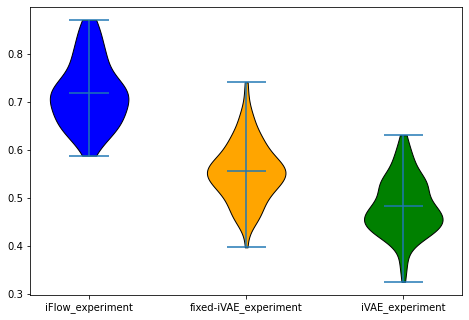
\includegraphics[width=0.5\textwidth]{Reproducibility_Challenge_2020/IMG/scores/violin_plot_fixed.png} 
    \caption{Alternative visualisation of the MCC scores obtained by the models, including the fixed iVAE.} 
    \label{fig:violinplot} 
\end{figure}

\begin{figure}[ht]
    \centering
    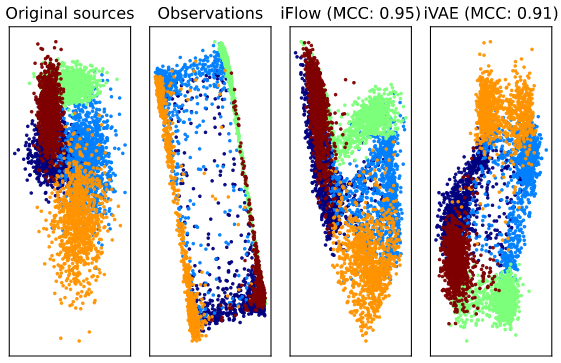
\includegraphics[width=0.5\textwidth]{Reproducibility_Challenge_2020/IMG/2D_perf/2D_performance_fixed_iVAE.png} 
    \caption{Visualisation of 2D-cases, comparing iFlow to the fixed version of iVAE.} 
    \label{fig:fixedMCCscores} 
\end{figure}

\begin{figure}[!htbp]
    \centering
    \begin{minipage}[b]{\textwidth}
        \centering
       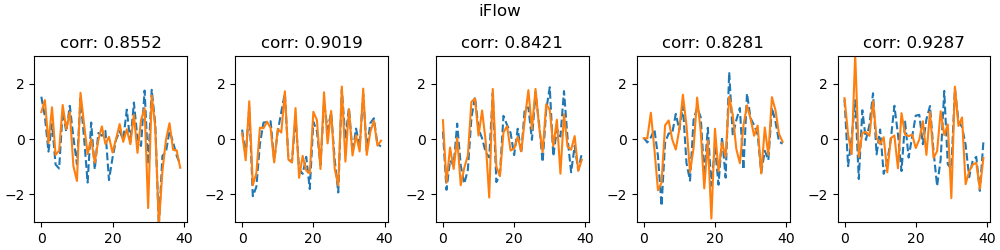
\includegraphics[width=0.8\textwidth]{Reproducibility_Challenge_2020/IMG/latent_corr/best_iFlow_42.png}
    \end{minipage}
    \begin{minipage}[b]{\textwidth}
    \centering
       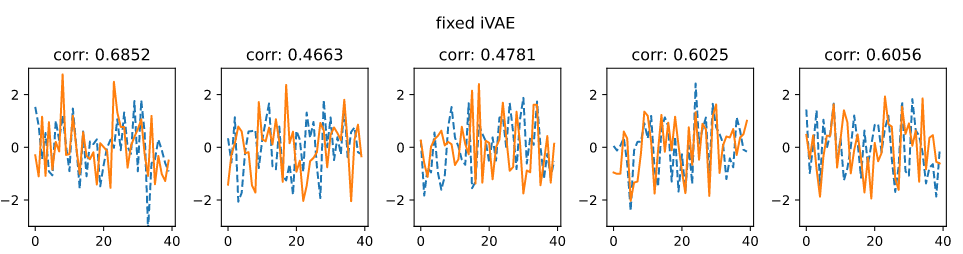
\includegraphics[width=0.8\textwidth]{Reproducibility_Challenge_2020/IMG/latent_corr/fixed_iVAE_42.png}
    \end{minipage}
    \caption{Comparison of the latent variables recovered by the models (orange lines) to the true latent variables (dashed blue lines) for individual dimensions. This figure shows results for the seed that resulted in the best iFlow performance.}
    \label{fig:latentcorr_fixed1}
\end{figure}

\begin{figure}[!htbp]
    \centering
    \begin{minipage}[b]{\textwidth}
        \centering
       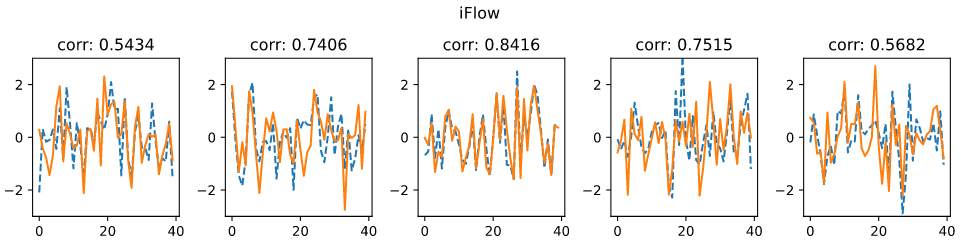
\includegraphics[width=0.8\textwidth]{Reproducibility_Challenge_2020/IMG/latent_corr/iFlow_X.png}
    \end{minipage}
    \begin{minipage}[b]{\textwidth}
    \centering
       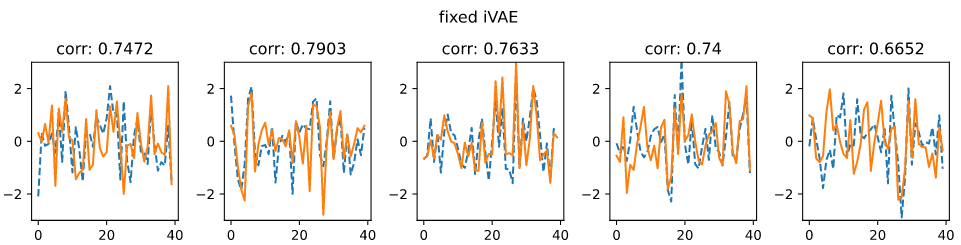
\includegraphics[width=0.8\textwidth]{Reproducibility_Challenge_2020/IMG/latent_corr/best_fixed_iVAE_X.png}
    \end{minipage}
    \caption{Comparison of the latent variables recovered by the models (orange lines) to the true latent variables (dashed blue lines) for individual dimensions. This figure shows results for the seed that resulted in the best fixed iVAE performance.}
    \label{fig:latentcorr_fixed2}
\end{figure}


\medskip

% \bibliography{ref}
\documentclass{article}

% if you need to pass options to natbib, use, e.g.:
%     \PassOptionsToPackage{numbers, compress}{natbib}
% before loading neurips_2019

% ready for submission
% \usepackage{neurips_2019}

% to compile a preprint version, e.g., for submission to arXiv, add add the
% [preprint] option:
    \usepackage[preprint]{neurips_2019}

% to compile a camera-ready version, add the [final] option, e.g.:
% \usepackage[final]{neurips_2019}

% to avoid loading the natbib package, add option nonatbib:
%     \usepackage[nonatbib]{neurips_2019}

\usepackage[utf8]{inputenc} % allow utf-8 input
\usepackage[T1]{fontenc}    % use 8-bit T1 fonts
\usepackage{hyperref}       % hyperlinks
\usepackage{url}            % simple URL typesetting
\usepackage{booktabs}       % professional-quality tables
\usepackage{caption}

% \DeclareCaptionLabelFormat{andtable}{#1~#2  \&  \tablename~\thetable}
\DeclareCaptionLabelFormat{andfigure}{#1~#2  \&  \figurename~\thefigure}

% Table and figure side by side
\usepackage{tabularx}
\usepackage[export]{adjustbox}

\usepackage{multirow}
\usepackage{comment}
\usepackage{makecell}
\usepackage{amsmath}
\usepackage{amsfonts}       % blackboard math symbols
\usepackage{nicefrac}       % compact symbols for 1/2, etc.
\usepackage{microtype}      % microtypography
\usepackage{graphicx}      % images
\usepackage[english]{babel}
\bibliographystyle{plainnat}

\usepackage[dvipsnames]{xcolor}
\usepackage[normalem]{ulem}
\newif{\ifhidecomments}

% set \hidecommentsfalse to see comments
\hidecommentstrue
% \hidecommentsfalse
\ifhidecomments
    \newcommand{\jdcomment}[1]{}
    \newcommand{\vscomment}[1]{} 
    % \newcommand{\vscomment}[1]{\textcolor{red}{[#1 ({\bf Varun})]}} 
    \newcommand{\resolved}[1]{}
\else
    \newcommand{\jdcomment}[1]{\textcolor{teal}{[#1 ({\bf Organisers})]}} 
    \newcommand{\vscomment}[1]{\textcolor{red}{[#1 ({\bf Varun})]}} 
    \newcommand{\resolved}[1]{} 
\fi

% Table & figure caption spacing
\newcommand{\tableaboveskip}{7pt}
\newcommand{\tablebelowskip}{0pt}
\newcommand{\figureaboveskip}{0pt}
\newcommand{\figurebelowskip}{7pt}

% ResNet-50 table
\newcommand{\blocka}[2]{\multirow{3}{*}{\(\left[\begin{array}{c}\text{3$\times$3, #1}\\[-.1em] \text{3$\times$3, #1} \end{array}\right]\)$\times$#2}
}

\newcommand{\blockb}[3]{\multirow{3}{*}{\(\left[\begin{array}{c}\text{1$\times$1, #2}\\[-.1em] \text{3$\times$3, #2}\\[-.1em] \text{1$\times$1, #1}\end{array}\right]\)$\times$#3}
}


\title{[Supplementary] \\Reproducibility Report \\Rigging the Lottery: Making All Tickets Winners}

% The \author macro works with any number of authors. There are two commands
% used to separate the names and addresses of multiple authors: \And and \AND.
%
% Using \And between authors leaves it to LaTeX to determine where to break the
% lines. Using \AND forces a line break at that point. So, if LaTeX puts 3 of 4
% authors names on the first line, and the last on the second line, try using
% \AND instead of \And before the third author name.

\author{%
  Varun Sundar \\
  University of Wisconsin Madison\\
  \texttt{vsundar4@wisc.edu} \\
  % examples of more authors
   \And
   Rajat Vadiraj Dwaraknath \\
   Stanford University \\
   \texttt{rajatvd@gmail.com} \\
}

\begin{document}

\maketitle


\section{Architecture Specific Details---ResNet-50 on CIFAR100}

\begin{table}[ht]
\captionsetup{aboveskip=\tableaboveskip,belowskip=\tablebelowskip}
\caption{\textbf{ResNet-50 architecture used on CIFAR100}. Building blocks are shown in brackets, with the numbers of blocks stacked. Downsampling is performed by conv3\_1, conv4\_1, and conv5\_1 with a stride of 2.
}
\label{tab:architecture}
\centering
\begin{tabular}{c c c}
    \toprule
    Layer Name & Output Size & ResNet-50 \\
    \midrule
    
    conv1 & 32$\times$32 & {3$\times$3, 64, no stride}\\
    \midrule
    
    \multirow{3}{*}{conv2\_x} & \multirow{3}{*}{32$\times$32} 
    & \blockb{256}{64}{3} \\
    &  &  \\
    &  &  \\
    \midrule
    
    \multirow{3}{*}{conv3\_x} &  \multirow{3}{*}{16$\times$16}  
    & \blockb{512}{128}{4} \\
    &  &  \\
    &  &  \\
    \midrule
    
    \multirow{3}{*}{conv4\_x} & \multirow{3}{*}{8$\times$8}  
    & \blockb{1024}{256}{6} \\
      &  &  \\
      &  &  \\
    \midrule
    
    \multirow{3}{*}{conv5\_x} & \multirow{3}{*}{4$\times$4}  
    & \blockb{2048}{512}{3} \\
      &  &   \\
      &  &   \\
    \midrule
    
    & 1$\times$1  & {average pool, 100-d fc, softmax} \\
    \midrule
    
    \multicolumn{2}{c}{FLOPs} & 2.59e9 \\
    \bottomrule
\end{tabular}
\end{table}

We use a variant of the originally proposed ResNet architecture (\citet{He_2016_CVPR}). Particularly, we replace the initial $7 \times 7$ conv layer with a $3 \times 3$ conv layer. Here, ``conv layer'' refers to convolution followed by batchnorm (\citet{ioffe2015batch}) and ReLU activation. This is intended to not excessively downsample the image---CIFAR-100 (\citet{Krizhevsky09learningmultiple}) has images of dimensions $32 \times 32$, compared to Imagenet's (\citet{ILSVRC15}) $224 \times 224$. Each block used (conv2\_x, conv3\_x, etc.) is a bottleneck block, and uses the conv-batchnorm-ReLU ordering. 
\section{FLOP Counting Procedure}

Following \citet{rigl}, we base our counting procedure on the Micronet Challenge\footnote{https://micronet-challenge.github.io/}, which was conducted as a part of NeurIPS 2019. Support for unstructured sparsity is assumed while computing the number of additions and multiplication operations. The sum of these two gives us the theoretical FLOPs for a single forward pass through the model. \\

Concretely, let the FLOPs required for a forward pass through a dense model be $f_d$ and the corresponding for a sparse model (or small-dense model) be $f_s$. Then, the FLOPs for training a dense model are $3f_d$---since the backward pass involves computing gradients with respect to each weight and activation. $f_s$ can be computed for a model given its sparsity distribution via the counting procedure. The FLOPs required to train a sparse model depend on the technique used, as detailed below.

\subsection{Inference FLOPs}

\subsubsection{Small-Dense, RigL, SET, Static} These methods involve constant layer-wise sparsity throughout training, hence the FLOP count can be determined during any step. The FLOP count for Random initialized models are $(1-s)$ times the Dense FLOPs.

\subsubsection{SNFS, Pruning} Both methods involve varying layer-wise sparsity during training, and hence non-constant FLOP consumption. The final weights are used to determine inference FLOPs in this case.

\subsection{Train FLOPs}

\subsubsection{Small-Dense, Static} Dense gradients are not required by these models, and hence have a train FLOP count of $3f_s$.

\subsubsection{SET} Dense gradients are not required, and random growth can be implemented quite efficiently. Thus, the train FLOP count is $3f_s$.

\subsubsection{RigL} Dense gradients are required only every $\Delta T$ steps, hence the corresponding train FLOP count is: $\frac{3\Delta Tf_s + 2f_s + f_d }{\Delta T + 1}$. We note that since $\Delta T$ is typically set between 100--1000, the preceding expression is quite close to $3f_s$.

\subsubsection{SNFS} Dense gradients are required at each training step, resulting in $2f_s + f_d$ FLOPs consumed at each step. Since the sparse FLOP count varies as we train, the average FLOP count is: $2\mathbb{E}[f_{s,t}] + f_d$, where $f_{s,t}$ is the sparse inference FLOPs at train step $t$.

\subsubsection{Pruning} Does not require dense gradients, but the sparsity increases smoothly from $0\%$ to the target value as we train. The FLOP consumption here is $3\mathbb{E}[f_{s,t}]$, , where $f_{s,t}$ is the sparse inference FLOPs at train step $t$.\\

To determine $\mathbb{E}[f_{s,t}]$, we compute a running average of the FLOP consumption after every epoch. Notably, we find that the inference cost of Pruning is often close to a Random initialized sparse network, while SNFS, regardless of initiazation, is compute-intensive.
\subsection{Hyperparameter Tuning}\label{hyperparameter-tuning}

\begin{table}[th]
    \captionsetup{aboveskip=\tableaboveskip,belowskip=\tablebelowskip}
    \caption{\textbf{Reference vs Optimal $(\alpha, \Delta T)$ on CIFAR-10.} Optimal hyperparameters are obtained by tuning with a TPE sampler in Optuna. The difference between the reference and optimal performance is small, indicating that there is not a significant benefit in tuning $(\alpha, \Delta T)$ individually for each initialization and sparsity configuration.}
    \label{tab:effect-alpha-deltaT}
    \centering
    
    \begin{tabular}{ c c  cc  cc}
    \toprule
    \multirow{3}{*}{\textbf{Initialization}} & \textbf{Density} & 
    \multicolumn{2}{c}{\textbf{Reference}} & \multicolumn{2}{c}{\textbf{Optimal}} \\
    \cmidrule(lr){2-2} \cmidrule(lr){3-4} \cmidrule(lr){5-6}
    {} & {$(1-s)$} & 
    {$(\alpha, \Delta T)$} & \makecell{Accuracy $\uparrow$ \\ (Test)} & 
    {$(\alpha, \Delta T)$} & \makecell{Accuracy $\uparrow$ \\ (Test)} \\
    \midrule
    
    Random & 0.1 & 
    {0.3, 100} & {91.7 $\pm$ 0.18} &  
    {0.197, 50} & \textbf{91.8 $\pm$ 0.17} \\
    
    Random & 0.2 & 
    {0.3, 100} & {92.6 $\pm$ 0.10} &  
    {0.448, 150} & \textbf{92.8 $\pm$ 0.16} \\
    
    Random & 0.5 & 
    {0.3, 100} & \textbf{93.3 $\pm$ 0.07} &  
    {0.459, 550} & \textbf{93.3 $\pm$ 0.18} \\
    \midrule
    
    ERK & 0.1 & 
    {0.3, 100} & \textbf{92.4 $\pm$ 0.06} &  
    {0.416, 200} & \textbf{92.4 $\pm$ 0.23} \\
    
    ERK & 0.2 & 
    {0.3, 100} & \textbf{93.1 $\pm$ 0.09} &  
    {0.381, 950} & \textbf{93.1 $\pm$ 0.21} \\
    
    ERK & 0.5 & 
    {0.3, 100} & {93.4 $\pm$ 0.14} &  
    {0.287, 500} & \textbf{93.8 $\pm$ 0.06} \\
    \hline

    \end{tabular}
    
    \label{tab:replication_verify}
\end{table}

\subsubsection{$(\alpha, \Delta T)$ vs Sparsities} To understand the impact of the two additional hyperparameters included in \textit{RigL}, we use a Tree of Parzen Estimator (TPE sampler, \citet{TPE_Bergstra}) via Optuna to tune $(\alpha, \Delta T)$. We do this for sparsities $(1 - s) \in \{0.1,0.2,0.5\}$, and a fixed learning rate of $0.1$. Additionally, we set the sampling domain for $\alpha$ and $\Delta T$ as $[0.1,0.6]$ and $\{50,100, 150,...,1000\}$ respectively. We use 15 trials for each sparsity value, with our objective function as the validation accuracy averaged across 3 random seeds.

\begin{figure}[!b]
    \centering
    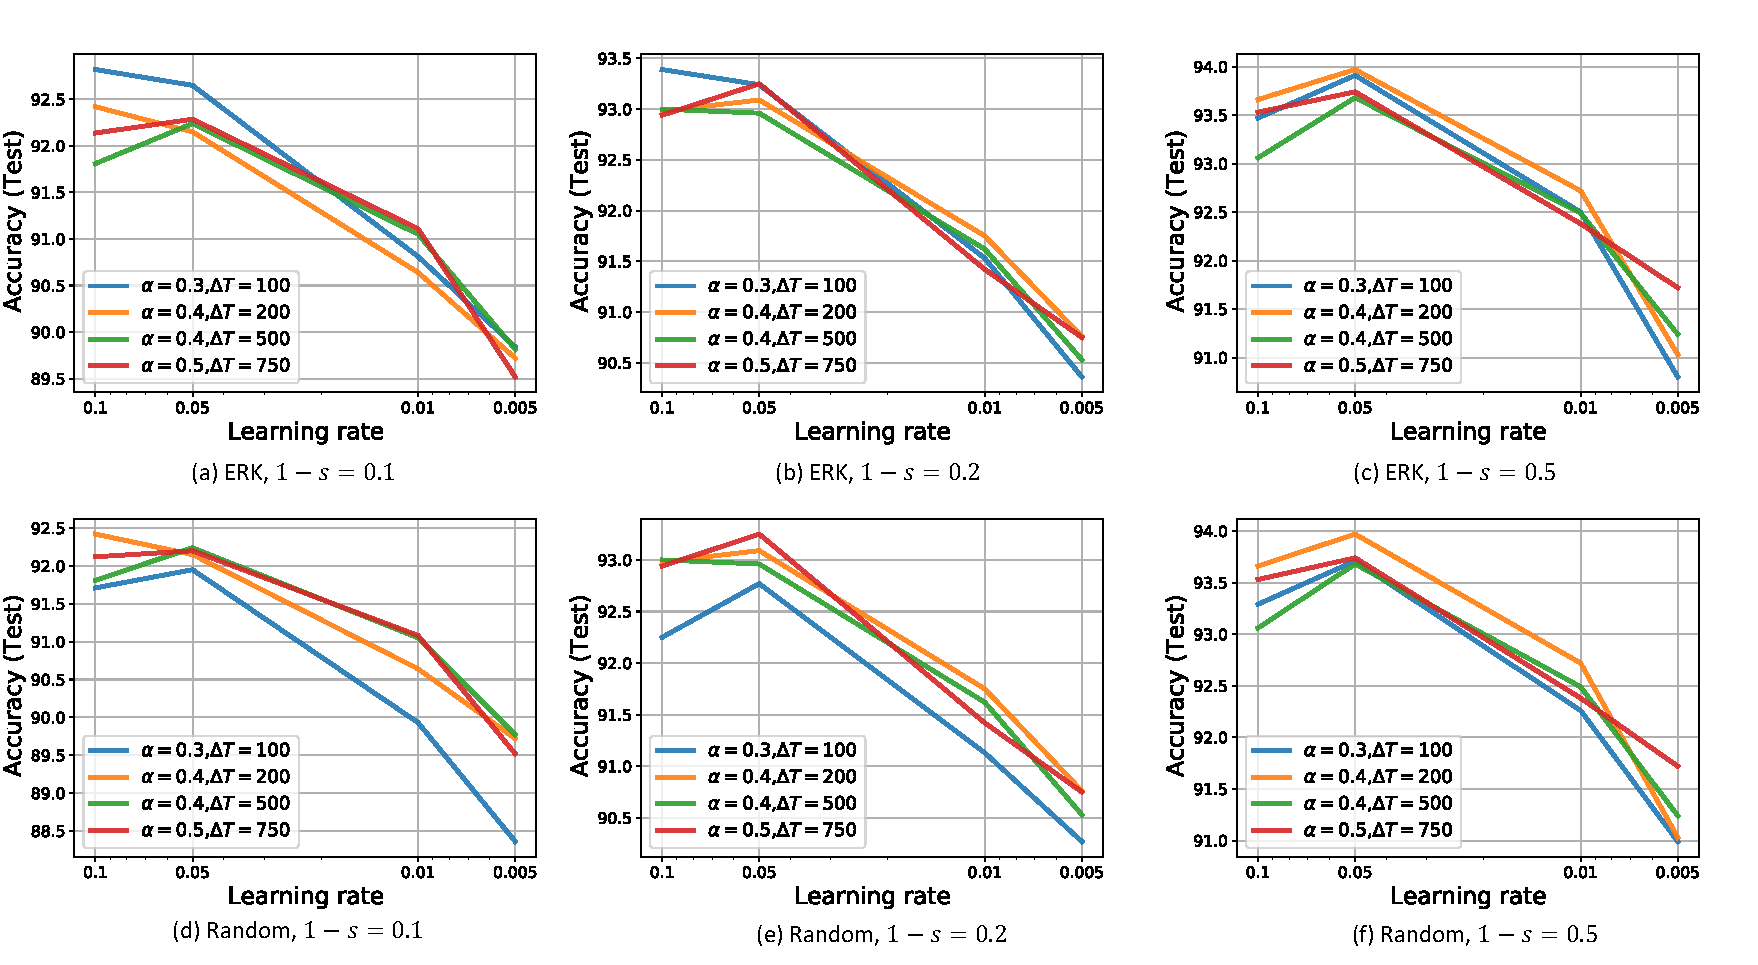
\includegraphics[width=\textwidth]{../openreview/figs/lr_sweep.pdf}
    \captionsetup{aboveskip=\figureaboveskip,belowskip=\figurebelowskip}
    \caption{\textbf{Learning Rate vs Sparsity on CIFAR-10.} Runs using a learning rate $> 0.1$ do not converge and are not plotted here. There is little benefit in tuning the learning rate for each sparsity, and $0.1, 0.05$ are good choices overall.}
    \label{fig:lr-sweep}
\end{figure}

Table \ref{tab:effect-alpha-deltaT} shows the test accuracies of tuned hyperparameters. While the reference hyperparameters (original authors, $\alpha=0.3, \Delta T=100$) differ from the obtained optimal hyperparameters, the difference in performance is marginal, especially for ERK initialization. This in agreement with the original paper, which finds $\alpha \in \{0.3, 0.5\}, \Delta T = 100$ to be suitable choices. We include contour plots detailing the hyperparameter trial space in the supplementary material.

\subsubsection{Learning Rate vs Sparsities} We further examine if the final performance improves by tuning the learning rate ($\eta$) individually for each sparsity-initialization pair. We employ a grid search over $\eta \in \{0.1,0.05,0.01,0.005\}$ and $(\alpha, \Delta T) \in \{(0.3, 100), (0.4,200), (0.4, 500), (0.5, 750)\}$. As seen in Figure \ref{fig:lr-sweep}, $\eta = 0.1$ and $\eta = 0.05$ are close to optimal values for a wide range of sparsities and initializations. Since these learning rates also correspond to good choices for the Dense baseline, one can employ similar values when training with \textit{RigL}.


\section{Dynamic Structured Sparsity}\label{structured-sparsity}

\begin{table}[h]
    \captionsetup{aboveskip=\tableaboveskip,belowskip=\tablebelowskip}
    \caption{\textbf{Modifying \textit{RigL} for structured sparsity, compared on CIFAR-10 and CIFAR-100 datasets.} \textit{RigL}-struct fails to match the accuracy of \textit{RigL} and just matches Small-Dense in performance. }
    \centering
    
    \resizebox{\textwidth}{!}{%
    \begin{tabular}{ c cc cc cc cc}
     \toprule
    \multirow{3}{*}{\textbf{Method}} & 
    \multicolumn{4}{c}{\textbf{CIFAR-10}} & \multicolumn{4}{c}{\textbf{CIFAR-100}} \\
    \cmidrule(lr){2-5} \cmidrule(lr){6-9}
    
    {} &
    \multicolumn{2}{c}{$1 - s=0.1$} & \multicolumn{2}{c}{$1 - s=0.2$} &
    \multicolumn{2}{c}{$1 - s=0.1$} & \multicolumn{2}{c}{$1 - s=0.2$} \\
    \cmidrule(lr){2-5} \cmidrule(lr){4-5} \cmidrule(lr){6-7} \cmidrule(lr){8-9}
    
    {} & 
    \makecell{Accuracy $\uparrow$ \\ (Test)}  & \makecell{Wall Time $\downarrow$} &
    \makecell{Accuracy $\uparrow$ \\ (Test)}  & \makecell{Wall Time $\downarrow$}  &
    \makecell{Accuracy $\uparrow$ \\ (Test)}  & \makecell{Wall Time $\downarrow$} &
    \makecell{Accuracy $\uparrow$ \\ (Test)}  & \makecell{Wall Time $\downarrow$} \\
    \midrule
    
    {Small-Dense} &
    {89.0 $\pm$ 0.35} & {0.11x} & 
    {91.0 $\pm$ 0.07} & {0.20x} &
    {70.8 $\pm$ 0.22} & {0.11x} & 
    {72.6$\pm$ 0.93} & {0.20x} \\
    
    \midrule
    
    \multicolumn{9}{c}{Random Initialization} \\
    \midrule
    
    {RigL} &
    {91.7 $\pm$ 0.18} & {1.0x} &
    {92.9 $\pm$ 0.10} & {1.0x} &
    {71.8 $\pm$ 0.33} & {1.0x} &
    {73.5 $\pm$ 0.04} & {1.0x} \\
    
    {RigL-Struct} &
    {87.0 $\pm$ 0.09} & {0.10x} &
    {90.4 $\pm$ 0.27} & {0.20x} &
    {69.1 $\pm$ 0.11} & {0.10x} &
    {71.9 $\pm$ 0.13} & {0.20x} \\
    
    \midrule
    \multicolumn{9}{c}{ERK Initialization} \\
    \midrule
    
    {RigL} &
    {92.4 $\pm$ 0.06} & {1.0x} &
    {93.1 $\pm$ 0.09} & {1.0x} &
    {72.6 $\pm$ 0.37} & {1.0x} &
    {73.4 $\pm$ 0.15} & {1.0x} \\
    
    {RigL-Struct} &
    {89.6 $\pm$ 0.16} & {0.17x} &
    {91.3 $\pm$ 0.18} & {0.35x} &
    {71.1 $\pm$ 0.15} & {0.23x} &
    {72.9 $\pm$ 0.08} & {0.38x} \\
    \bottomrule
    
    \end{tabular}%
    }
    
    \label{tab:structured-sparsity}
\end{table}

Present hardware accelerators lack efficient implementations for unstructured sparsity. As a result, in practice, the reduced FLOP requirement of sparse methods rarely translate to wall-clock improvements. In comparison, there are efficient implementations available for structured (or block) sparsity which reach theoretical speedups (\citet{gray2017gpu,Vooturi_2019_ICCV}).\\

Motivated by this, we try modifying \textit{RigL} to explicitly work on structured sparsity. We promote channel sparsity for convolutional layers and keep fully connected layers dense. Mask update steps also operate at the channel level, based on \textit{RigL}'s growth and pruning criterion. We name this method as \textit{RigL}-struct. Such an approach is enticing, as we can remove masked-out channels, and obtain practical speedups on accelerators without needing support for unstructured sparsity.\\

Unfortunately, \textit{RigL}-struct does not preserve the performance of originally proposed \textit{RigL} (Table \ref{tab:structured-sparsity}). In fact, it performs only as good as Small-Dense models, which negates the motivation behind such an experiment---Small-Dense models already achieve the intended speedups.

\medskip

% \bibliography{ref}
\documentclass{article}

% if you need to pass options to natbib, use, e.g.:
%     \PassOptionsToPackage{numbers, compress}{natbib}
% before loading neurips_2019

% ready for submission
% \usepackage{neurips_2019}

% to compile a preprint version, e.g., for submission to arXiv, add add the
% [preprint] option:
    \usepackage[preprint]{neurips_2019}

% to compile a camera-ready version, add the [final] option, e.g.:
% \usepackage[final]{neurips_2019}

% to avoid loading the natbib package, add option nonatbib:
%     \usepackage[nonatbib]{neurips_2019}

\usepackage[utf8]{inputenc} % allow utf-8 input
\usepackage[T1]{fontenc}    % use 8-bit T1 fonts
\usepackage{hyperref}       % hyperlinks
\usepackage{url}            % simple URL typesetting
\usepackage{booktabs}       % professional-quality tables
\usepackage{caption}

% \DeclareCaptionLabelFormat{andtable}{#1~#2  \&  \tablename~\thetable}
\DeclareCaptionLabelFormat{andfigure}{#1~#2  \&  \figurename~\thefigure}

% Table and figure side by side
\usepackage{tabularx}
\usepackage[export]{adjustbox}

\usepackage{multirow}
\usepackage{comment}
\usepackage{makecell}
\usepackage{amsmath}
\usepackage{amsfonts}       % blackboard math symbols
\usepackage{nicefrac}       % compact symbols for 1/2, etc.
\usepackage{microtype}      % microtypography
\usepackage{graphicx}      % images
\usepackage[english]{babel}
\bibliographystyle{plainnat}

\usepackage[dvipsnames]{xcolor}
\usepackage[normalem]{ulem}
\newif{\ifhidecomments}

% set \hidecommentsfalse to see comments
\hidecommentstrue
% \hidecommentsfalse
\ifhidecomments
    \newcommand{\jdcomment}[1]{}
    \newcommand{\vscomment}[1]{} 
    % \newcommand{\vscomment}[1]{\textcolor{red}{[#1 ({\bf Varun})]}} 
    \newcommand{\resolved}[1]{}
\else
    \newcommand{\jdcomment}[1]{\textcolor{teal}{[#1 ({\bf Organisers})]}} 
    \newcommand{\vscomment}[1]{\textcolor{red}{[#1 ({\bf Varun})]}} 
    \newcommand{\resolved}[1]{} 
\fi

% Table & figure caption spacing
\newcommand{\tableaboveskip}{7pt}
\newcommand{\tablebelowskip}{0pt}
\newcommand{\figureaboveskip}{0pt}
\newcommand{\figurebelowskip}{7pt}

% ResNet-50 table
\newcommand{\blocka}[2]{\multirow{3}{*}{\(\left[\begin{array}{c}\text{3$\times$3, #1}\\[-.1em] \text{3$\times$3, #1} \end{array}\right]\)$\times$#2}
}

\newcommand{\blockb}[3]{\multirow{3}{*}{\(\left[\begin{array}{c}\text{1$\times$1, #2}\\[-.1em] \text{3$\times$3, #2}\\[-.1em] \text{1$\times$1, #1}\end{array}\right]\)$\times$#3}
}


\title{[Supplementary] \\Reproducibility Report \\Rigging the Lottery: Making All Tickets Winners}

% The \author macro works with any number of authors. There are two commands
% used to separate the names and addresses of multiple authors: \And and \AND.
%
% Using \And between authors leaves it to LaTeX to determine where to break the
% lines. Using \AND forces a line break at that point. So, if LaTeX puts 3 of 4
% authors names on the first line, and the last on the second line, try using
% \AND instead of \And before the third author name.

\author{%
  Varun Sundar \\
  University of Wisconsin Madison\\
  \texttt{vsundar4@wisc.edu} \\
  % examples of more authors
   \And
   Rajat Vadiraj Dwaraknath \\
   Stanford University \\
   \texttt{rajatvd@gmail.com} \\
}

\begin{document}

\maketitle


\section{Architecture Specific Details---ResNet-50 on CIFAR100}

\begin{table}[ht]
\captionsetup{aboveskip=\tableaboveskip,belowskip=\tablebelowskip}
\caption{\textbf{ResNet-50 architecture used on CIFAR100}. Building blocks are shown in brackets, with the numbers of blocks stacked. Downsampling is performed by conv3\_1, conv4\_1, and conv5\_1 with a stride of 2.
}
\label{tab:architecture}
\centering
\begin{tabular}{c c c}
    \toprule
    Layer Name & Output Size & ResNet-50 \\
    \midrule
    
    conv1 & 32$\times$32 & {3$\times$3, 64, no stride}\\
    \midrule
    
    \multirow{3}{*}{conv2\_x} & \multirow{3}{*}{32$\times$32} 
    & \blockb{256}{64}{3} \\
    &  &  \\
    &  &  \\
    \midrule
    
    \multirow{3}{*}{conv3\_x} &  \multirow{3}{*}{16$\times$16}  
    & \blockb{512}{128}{4} \\
    &  &  \\
    &  &  \\
    \midrule
    
    \multirow{3}{*}{conv4\_x} & \multirow{3}{*}{8$\times$8}  
    & \blockb{1024}{256}{6} \\
      &  &  \\
      &  &  \\
    \midrule
    
    \multirow{3}{*}{conv5\_x} & \multirow{3}{*}{4$\times$4}  
    & \blockb{2048}{512}{3} \\
      &  &   \\
      &  &   \\
    \midrule
    
    & 1$\times$1  & {average pool, 100-d fc, softmax} \\
    \midrule
    
    \multicolumn{2}{c}{FLOPs} & 2.59e9 \\
    \bottomrule
\end{tabular}
\end{table}

We use a variant of the originally proposed ResNet architecture (\citet{He_2016_CVPR}). Particularly, we replace the initial $7 \times 7$ conv layer with a $3 \times 3$ conv layer. Here, ``conv layer'' refers to convolution followed by batchnorm (\citet{ioffe2015batch}) and ReLU activation. This is intended to not excessively downsample the image---CIFAR-100 (\citet{Krizhevsky09learningmultiple}) has images of dimensions $32 \times 32$, compared to Imagenet's (\citet{ILSVRC15}) $224 \times 224$. Each block used (conv2\_x, conv3\_x, etc.) is a bottleneck block, and uses the conv-batchnorm-ReLU ordering. 
\section{FLOP Counting Procedure}

Following \citet{rigl}, we base our counting procedure on the Micronet Challenge\footnote{https://micronet-challenge.github.io/}, which was conducted as a part of NeurIPS 2019. Support for unstructured sparsity is assumed while computing the number of additions and multiplication operations. The sum of these two gives us the theoretical FLOPs for a single forward pass through the model. \\

Concretely, let the FLOPs required for a forward pass through a dense model be $f_d$ and the corresponding for a sparse model (or small-dense model) be $f_s$. Then, the FLOPs for training a dense model are $3f_d$---since the backward pass involves computing gradients with respect to each weight and activation. $f_s$ can be computed for a model given its sparsity distribution via the counting procedure. The FLOPs required to train a sparse model depend on the technique used, as detailed below.

\subsection{Inference FLOPs}

\subsubsection{Small-Dense, RigL, SET, Static} These methods involve constant layer-wise sparsity throughout training, hence the FLOP count can be determined during any step. The FLOP count for Random initialized models are $(1-s)$ times the Dense FLOPs.

\subsubsection{SNFS, Pruning} Both methods involve varying layer-wise sparsity during training, and hence non-constant FLOP consumption. The final weights are used to determine inference FLOPs in this case.

\subsection{Train FLOPs}

\subsubsection{Small-Dense, Static} Dense gradients are not required by these models, and hence have a train FLOP count of $3f_s$.

\subsubsection{SET} Dense gradients are not required, and random growth can be implemented quite efficiently. Thus, the train FLOP count is $3f_s$.

\subsubsection{RigL} Dense gradients are required only every $\Delta T$ steps, hence the corresponding train FLOP count is: $\frac{3\Delta Tf_s + 2f_s + f_d }{\Delta T + 1}$. We note that since $\Delta T$ is typically set between 100--1000, the preceding expression is quite close to $3f_s$.

\subsubsection{SNFS} Dense gradients are required at each training step, resulting in $2f_s + f_d$ FLOPs consumed at each step. Since the sparse FLOP count varies as we train, the average FLOP count is: $2\mathbb{E}[f_{s,t}] + f_d$, where $f_{s,t}$ is the sparse inference FLOPs at train step $t$.

\subsubsection{Pruning} Does not require dense gradients, but the sparsity increases smoothly from $0\%$ to the target value as we train. The FLOP consumption here is $3\mathbb{E}[f_{s,t}]$, , where $f_{s,t}$ is the sparse inference FLOPs at train step $t$.\\

To determine $\mathbb{E}[f_{s,t}]$, we compute a running average of the FLOP consumption after every epoch. Notably, we find that the inference cost of Pruning is often close to a Random initialized sparse network, while SNFS, regardless of initiazation, is compute-intensive.
\subsection{Hyperparameter Tuning}\label{hyperparameter-tuning}

\input{../openreview/tables/alpha_deltaT.tex}

\subsubsection{$(\alpha, \Delta T)$ vs Sparsities} To understand the impact of the two additional hyperparameters included in \textit{RigL}, we use a Tree of Parzen Estimator (TPE sampler, \citet{TPE_Bergstra}) via Optuna to tune $(\alpha, \Delta T)$. We do this for sparsities $(1 - s) \in \{0.1,0.2,0.5\}$, and a fixed learning rate of $0.1$. Additionally, we set the sampling domain for $\alpha$ and $\Delta T$ as $[0.1,0.6]$ and $\{50,100, 150,...,1000\}$ respectively. We use 15 trials for each sparsity value, with our objective function as the validation accuracy averaged across 3 random seeds.

\input{../openreview/figs/lr_sweep.tex}

Table \ref{tab:effect-alpha-deltaT} shows the test accuracies of tuned hyperparameters. While the reference hyperparameters (original authors, $\alpha=0.3, \Delta T=100$) differ from the obtained optimal hyperparameters, the difference in performance is marginal, especially for ERK initialization. This in agreement with the original paper, which finds $\alpha \in \{0.3, 0.5\}, \Delta T = 100$ to be suitable choices. We include contour plots detailing the hyperparameter trial space in the supplementary material.

\subsubsection{Learning Rate vs Sparsities} We further examine if the final performance improves by tuning the learning rate ($\eta$) individually for each sparsity-initialization pair. We employ a grid search over $\eta \in \{0.1,0.05,0.01,0.005\}$ and $(\alpha, \Delta T) \in \{(0.3, 100), (0.4,200), (0.4, 500), (0.5, 750)\}$. As seen in Figure \ref{fig:lr-sweep}, $\eta = 0.1$ and $\eta = 0.05$ are close to optimal values for a wide range of sparsities and initializations. Since these learning rates also correspond to good choices for the Dense baseline, one can employ similar values when training with \textit{RigL}.


\section{Dynamic Structured Sparsity}\label{structured-sparsity}

\input{../openreview/supplementary_sections/table_structured_sparsity.tex}

Present hardware accelerators lack efficient implementations for unstructured sparsity. As a result, in practice, the reduced FLOP requirement of sparse methods rarely translate to wall-clock improvements. In comparison, there are efficient implementations available for structured (or block) sparsity which reach theoretical speedups (\citet{gray2017gpu,Vooturi_2019_ICCV}).\\

Motivated by this, we try modifying \textit{RigL} to explicitly work on structured sparsity. We promote channel sparsity for convolutional layers and keep fully connected layers dense. Mask update steps also operate at the channel level, based on \textit{RigL}'s growth and pruning criterion. We name this method as \textit{RigL}-struct. Such an approach is enticing, as we can remove masked-out channels, and obtain practical speedups on accelerators without needing support for unstructured sparsity.\\

Unfortunately, \textit{RigL}-struct does not preserve the performance of originally proposed \textit{RigL} (Table \ref{tab:structured-sparsity}). In fact, it performs only as good as Small-Dense models, which negates the motivation behind such an experiment---Small-Dense models already achieve the intended speedups.

\medskip

% \bibliography{ref}
\documentclass{article}

% if you need to pass options to natbib, use, e.g.:
%     \PassOptionsToPackage{numbers, compress}{natbib}
% before loading neurips_2019

% ready for submission
% \usepackage{neurips_2019}

% to compile a preprint version, e.g., for submission to arXiv, add add the
% [preprint] option:
    \usepackage[preprint]{neurips_2019}

% to compile a camera-ready version, add the [final] option, e.g.:
% \usepackage[final]{neurips_2019}

% to avoid loading the natbib package, add option nonatbib:
%     \usepackage[nonatbib]{neurips_2019}

\usepackage[utf8]{inputenc} % allow utf-8 input
\usepackage[T1]{fontenc}    % use 8-bit T1 fonts
\usepackage{hyperref}       % hyperlinks
\usepackage{url}            % simple URL typesetting
\usepackage{booktabs}       % professional-quality tables
\usepackage{caption}

% \DeclareCaptionLabelFormat{andtable}{#1~#2  \&  \tablename~\thetable}
\DeclareCaptionLabelFormat{andfigure}{#1~#2  \&  \figurename~\thefigure}

% Table and figure side by side
\usepackage{tabularx}
\usepackage[export]{adjustbox}

\usepackage{multirow}
\usepackage{comment}
\usepackage{makecell}
\usepackage{amsmath}
\usepackage{amsfonts}       % blackboard math symbols
\usepackage{nicefrac}       % compact symbols for 1/2, etc.
\usepackage{microtype}      % microtypography
\usepackage{graphicx}      % images
\usepackage[english]{babel}
\bibliographystyle{plainnat}

\usepackage[dvipsnames]{xcolor}
\usepackage[normalem]{ulem}
\newif{\ifhidecomments}

% set \hidecommentsfalse to see comments
\hidecommentstrue
% \hidecommentsfalse
\ifhidecomments
    \newcommand{\jdcomment}[1]{}
    \newcommand{\vscomment}[1]{} 
    % \newcommand{\vscomment}[1]{\textcolor{red}{[#1 ({\bf Varun})]}} 
    \newcommand{\resolved}[1]{}
\else
    \newcommand{\jdcomment}[1]{\textcolor{teal}{[#1 ({\bf Organisers})]}} 
    \newcommand{\vscomment}[1]{\textcolor{red}{[#1 ({\bf Varun})]}} 
    \newcommand{\resolved}[1]{} 
\fi

% Table & figure caption spacing
\newcommand{\tableaboveskip}{7pt}
\newcommand{\tablebelowskip}{0pt}
\newcommand{\figureaboveskip}{0pt}
\newcommand{\figurebelowskip}{7pt}

% ResNet-50 table
\newcommand{\blocka}[2]{\multirow{3}{*}{\(\left[\begin{array}{c}\text{3$\times$3, #1}\\[-.1em] \text{3$\times$3, #1} \end{array}\right]\)$\times$#2}
}

\newcommand{\blockb}[3]{\multirow{3}{*}{\(\left[\begin{array}{c}\text{1$\times$1, #2}\\[-.1em] \text{3$\times$3, #2}\\[-.1em] \text{1$\times$1, #1}\end{array}\right]\)$\times$#3}
}


\title{[Supplementary] \\Reproducibility Report \\Rigging the Lottery: Making All Tickets Winners}

% The \author macro works with any number of authors. There are two commands
% used to separate the names and addresses of multiple authors: \And and \AND.
%
% Using \And between authors leaves it to LaTeX to determine where to break the
% lines. Using \AND forces a line break at that point. So, if LaTeX puts 3 of 4
% authors names on the first line, and the last on the second line, try using
% \AND instead of \And before the third author name.

\author{%
  Varun Sundar \\
  University of Wisconsin Madison\\
  \texttt{vsundar4@wisc.edu} \\
  % examples of more authors
   \And
   Rajat Vadiraj Dwaraknath \\
   Stanford University \\
   \texttt{rajatvd@gmail.com} \\
}

\begin{document}

\maketitle


\input{supplementary_sections/architecture_details}
\input{supplementary_sections/flop_counting}
\input{supplementary_sections/hyperparameter_tuning}
\input{supplementary_sections/structured_sparsity}

\medskip

% \bibliography{ref}
\input{supplementary.bbl}

\end{document}


\end{document}


\end{document}


\end{document}
